%% main-en.tex — 紀要「文化情報学」LaTeX テンプレート 英語論文の使用例
%%
%% 英語で書く場合は、main.tex ではなくこのファイルを書き換えて原稿を作ります。
%% Overleaf では Menu → Main document を「main-en.tex」にしてください。
%% 「%」から行末まではコメント（PDF には出ません）。
%% Overleaf では Menu → Compiler を「LuaLaTeX」にしてください。

%% ---------------------------------------------------------------
%% 種別: [ ] の中の paper を書き換える（english は消さない）
%%   paper（Research Paper）/ note（Research Note）/ material（Material Introduction）/ review（Book Review）
%% ---------------------------------------------------------------
\documentclass[paper,english]{bunkajoho}

%% 文献データのファイル（このファイルと同じ場所に置く）
\addbibresource{sample.bib}

%% 表題・副題・著者名
\title{How to Use the \LaTeX{} Template for English Papers}
\subtitle{A Class File and Bibliography Style Based on the Submission Guidelines}   % 副題がなければこの行を消す
\author{Taro Doshisha and Hanako Bunka}                                              % 複数の著者は and や , で区切る

%% 要旨
\begin{abstract}
This paper describes how to use the \LaTeX{} template for papers written in English for the \textit{Journal of Culture and Information Science} (『文化情報学』).
The template is based on the submission guidelines revised on 7 December 2022.
The text itself serves as an example: it explains the title block, section numbering, figures and tables, equations, footnotes, and references in turn.
Open this file (main-en.tex), compare it with the PDF, and rewrite it to produce your manuscript.
\end{abstract}

\begin{document}
\maketitle   % ここにタイトル部（種別・表題・著者名・要旨）が出る

%% ---------------------------------------------------------------
%% 本文
%% ---------------------------------------------------------------
\section{Introduction}

The submission guidelines require that papers be prepared with \LaTeX{} or Microsoft Word using the style files provided by the editorial committee.
This template is an unofficial draft of the \LaTeX{} version.
This PDF is produced from main-en.tex, and you can write your manuscript by rewriting that file.
For matters not covered by the guidelines, papers in English follow the \textit{Publication Manual} of the American Psychological Association (APA).

The \verb|english| option in the first line of the file switches the type label, headings, captions, and citation parentheses to English.
Replace \verb|paper| in that line to change the type label at the top left of the first page.
\begin{verbatim}
\documentclass[paper,english]{bunkajoho}
\end{verbatim}
Use \verb|note| for a research note, \verb|material| for a material introduction, and \verb|review| for a book review.
Write the title, subtitle, and authors inside \verb|\title{...}|, \verb|\subtitle{...}|, and \verb|\author{...}|.
Write the abstract inside the \verb|abstract| environment.

The first page contains the title, type, authors, and abstract.
Do not add page numbers; the office adds them.

To start a new paragraph, leave a blank line.
A line break in the source alone does not start a new paragraph.

\section{Writing the Text}

\subsection{Sections and Subsections}

The text is divided into sections numbered as 1, 2.3, and 3.4.2.
In \LaTeX, write \verb|\section{Heading}|, \verb|\subsection{Heading}|, and \verb|\subsubsection{Heading}|; the numbers are added automatically.

\subsubsection{Notation}

Spell out an abbreviation at its first occurrence, followed by the abbreviation in parentheses, as in ``Large Language Model (LLM).''
Use \verb|``| and \verb|''| for double quotation marks in the source.

\subsubsection{Special Characters}

The characters \verb|% $ & # _ { } ~ ^ \| are used for \LaTeX{} commands and do not appear in the text as they are.
To print ``\%'' or ``\&,'' put a backslash before them, as in \verb|\%| and \verb|\&|.

\subsection{Equations}

Display equations on separate lines and number them consecutively.
Write a displayed equation inside the \verb|equation| environment.
\begin{equation}
  H(X) = -\sum_{i=1}^{n} p(x_i) \log_2 p(x_i)
  \label{eq:entropy}
\end{equation}
For equations within a sentence, enclose them in \verb|$|, as in \verb|$a/b$|, to obtain $a/b$, $\exp(x/y)$, or $\delta x/\delta t$.

If you name an equation with \verb|\label{eq:mi}|, you can refer to its number by writing \verb|Equation~\eqref{eq:mi}|, which gives ``Equation~\eqref{eq:mi}.''
The numbers are updated automatically when you add or remove equations.
\begin{equation}
  I(X;Y) = H(X) - H(X \mid Y)
  \label{eq:mi}
\end{equation}

\subsection{Notes}

Avoid notes as far as possible.\footnote{If a note is unavoidable, write it with \texttt{\textbackslash footnote\{...\}} like this. All notes are printed as footnotes.}

\section{Figures and Tables}

Number figures and tables consecutively, as in ``Figure 1'' and ``Table 1.''
Figure~\ref{fig:example} and Table~\ref{tab:example} show examples.
Name figures and tables with \verb|\label{...}| as well, and refer to them in the text as \verb|Figure~\ref{fig:example}|.
Figures and tables are placed automatically at the top or bottom of a column, so they may not appear where you wrote them in the source.

Embed figures and tables in the text of the manuscript submitted for review.
In the final manuscript after acceptance, leave the space for each figure blank and submit the figure data separately at a sufficient resolution.
When reproducing a figure or table from another source, obtain permission from the copyright holder in advance and cite the source.

%% 図: 画像ファイル（PNG, JPEG, PDF）をこのファイルと同じ場所に置き、ファイル名を書く。
%%   width=0.9\linewidth は「段の幅の 90%」
\begin{figure}[tb]
  \centering
  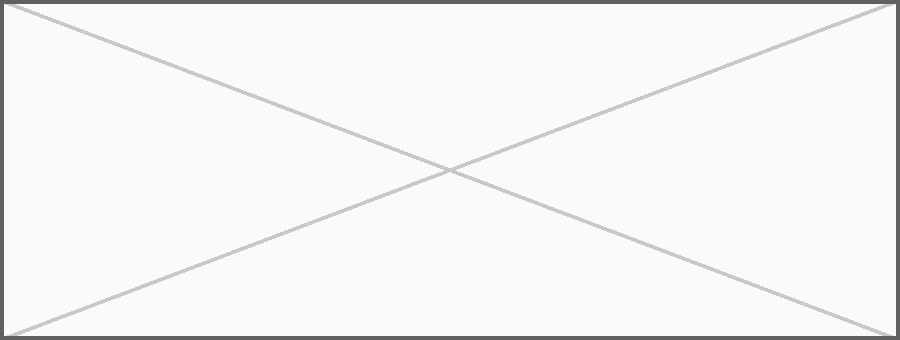
\includegraphics[width=0.9\linewidth]{figure1.png}
  \caption{An example figure}
  \label{fig:example}
\end{figure}

%% 表: {lrr} は各列の揃え（l 左, c 中央, r 右）。列は & で区切り、行末に \\ を書く。
%%   キャプションは表の上に置く。
\begin{table}[tb]
  \centering
  \caption{An example table}
  \label{tab:example}
  \begin{tabular}{lrr}
    \toprule
    Type & Count & Percent \\
    \midrule
    Research paper & 12 & 60.0 \\
    Research note & 5 & 25.0 \\
    Book review & 3 & 15.0 \\
    \bottomrule
  \end{tabular}
\end{table}

For a large figure or table spanning both columns, use \verb|figure*| or \verb|table*| instead of \verb|figure| or \verb|table| (Table~\ref{tab:cite} is an example).
In this case, the width \verb|\linewidth| is the width of both columns.

\section{References}

\subsection{Citations in the Text}

When citing a work in the text, give the author's surname followed by the year of publication.
In \LaTeX, write \verb|\citet{key}| or \verb|\citep{key}|, and the author and year are printed automatically in the required format.
The key is the name given to each work in the bibliography data (sample.bib).
Table~\ref{tab:cite} shows the examples in the guidelines and how to write them.

\begin{table*}[tb]
  \centering
  \caption{How to write citations and their output}
  \label{tab:cite}
  \footnotesize
  \begin{tabular}{ll}
    \toprule
    Source & Output \\
    \midrule
    \verb|\citet{gibson1979}| & \citet{gibson1979} \\
    \verb|\citep{saeki1990}| & \citep{saeki1990} \\
    \verb|\citet[123]{haugeland1987}| & \citet[123]{haugeland1987} \\
    \verb|Simon \citep*{simon1973,simon1981}| & Simon \citep*{simon1973,simon1981} \\
    \verb|\citep{simon1973,simon1981}| & \citep{simon1973,simon1981} \\
    \verb|\citet{cohen1990a}| & \citet{cohen1990a} \\
    \verb|\citep{cohen1990a,cohen1990b}| & \citep{cohen1990a,cohen1990b} \\
    \verb|\citep{anzai1992,joshi1981,minsky1975,minsky1986}| & \citep{anzai1992,joshi1981,minsky1975,minsky1986} \\
    \bottomrule
  \end{tabular}
\end{table*}

Use \verb|\citet| when the citation is part of the sentence, as in ``according to \citet{gibson1979}, \ldots,'' and \verb|\citep| otherwise, as in ``\ldots{} has been proposed \citep{saeki1990}.''
To give a page, write the page number in \verb|[ ]|, as in \verb|\citet[123]{haugeland1987}|.

\subsection{Writing Bibliography Data}

Collect the works you cite in a bib file such as sample.bib.
A journal article, for example, is written as follows.

\begin{small}
\begin{verbatim}
@article{miller1956,
  author       = {Miller, G. A.},
  year         = {1956},
  title        = {The Magical Number ...},
  journaltitle = {Psychological Review},
  volume       = {63},
  number       = {1},
  pages        = {81-97},
}
\end{verbatim}
\end{small}

The \verb|miller1956| in the first line is the key.
Write authors as ``Surname, Given names'' separated by \verb|and|.
For works in Japanese, add \verb|langid = {japanese}|, and give the romanized names in \verb|sortname| so that they are sorted correctly among works in English.
See sample.bib for books, edited volumes, and translations.

\subsection{Reference List}

Write \verb|\printbibliography| where the reference list should appear; it is printed under the heading ``References.''
Only the works cited in the text are listed, sorted alphabetically by the first author's surname without numbers, regardless of language.
The following sentence cites all the examples in the guidelines:
\citet{miller1956}, \citet{cohen1985}, Minsky \citep*{minsky1986,minsky1986b}, \citet{saeki1990}, \citet{minsky1975}, \citet{perrault1990b}, \citet{rosenschein1987}, and \citet{devins1981}.

\section{Conclusion}

This template is an unofficial draft.
The page size, number of characters per line, font sizes, and so on follow the typesetting of published papers.

%% 謝辞（不要なら消す）
\begin{acknowledgments}
Acknowledgments are placed after the text and before the references.
Write them inside the \verb|acknowledgments| environment.
\end{acknowledgments}

%% 文献リスト
\printbibliography

%% 付録（不要なら \appendix 以下を消す）
\appendix

\section{An Example Appendix}

Appendices are placed after the references.
Sections after \verb|\appendix| are numbered as ``Appendix A.''

\end{document}
